\documentclass[12pt,letterpaper,addpoints]{exam}
\usepackage[utf8]{inputenc}
\usepackage{amsmath}
\usepackage{amsfonts}
\usepackage{amssymb}
\usepackage{amsthm}
\usepackage{graphicx}
\usepackage{tabularx}
\usepackage[left=2cm,right=2cm,top=2cm,bottom=2cm]{geometry}
\usepackage{multicol}
\usepackage{multirow,array}
\usepackage{newtxtext,newtxmath}
\usepackage{lastpage}
\usepackage{enumitem}
\newcolumntype{Y}{>{\centering\arraybackslash}X}
\firstpageheader{}{}{
\includegraphics[scale=0.5]{BHCClogoBW.jpg}\hspace{-40pt}\vspace{-50pt}}
\firstpagefooter{}{}{Page \thepage ~of \pageref{LastPage}}
\runningheader{ \textsc{Math 181 First Exam Practice C}}{}{ \textsc{Fall 2018}}%{
\includegraphics[scale=.5]{BHCClogoBW.jpg}\vspace{-10pt}}%\hspace{-60pt}\vspace{-10pt}}
\runningheadrule
\runningfooter{}{}{Page \thepage ~of \pageref{LastPage}}
\renewcommand{\thequestion}{{\bf Q\arabic{question}}}
%\renewcommand{\questionlabel}{{\thequestion .}}
%\pointformat{\fbox{\themarginpoints \,pt}}
%\pointsinrightmargin
%\setlength{\rightpointsmargin}{1.5cm}
%\pointsinmargin
%\setlength{\marginpointssep}{10pt}

\begin{document}

\newcommand{\AND}{~\textsc{and}~}
\newcommand{\OR}{~\textsc{or}~}

\begin{center}
\text{ }\\
\vspace{40pt}
\textsc{{\Huge Math 181 First Exam Practice C}}\\\vspace{5pt}
\textsc{{\large Spring 2019}}\\
\vspace{60pt}
\makebox[\textwidth]{\large Name:\enspace\hrulefill}\\
\vspace{40pt}
\fbox{\fbox{\begin{minipage}{6in}
\vspace{0.2in}
\begin{itemize}
\item Write your {\bf full name} on the line above.
\item Show your work. Incorrect answers with work can receive partial credit.
\item Attempt every question; showing you understand the question earns some credit.
\item If you run out of room for an answer, continue on the back of the page. Before doing so, write ``see back'' with a circle around it.
\item You can use 1 page (front and back) of notes.
\item You can use (and probably need) a calculator.
\item You can use the Geogebra Scientific Calculator instead of a calculator. You need to put your phone on {\bf airplane mode} and then within the application, start {\bf exam mode}; you should see a green bar with a timer counting up.
\item If a question is confusing or ambiguous, please ask for clarification; however, you will not be told how to  answer the question.
\item {\bf Box your final answer}.
\item A formula sheet is attached to this test.
\vspace{0.2in}
\end{itemize}
\end{minipage}
\begin{minipage}{0.2in}\text{ }\end{minipage}}}
\vfill
Do not write in this grade table.\\
\gradetable[h][questions]\\
\vfill
\end{center}

%%%%%%%%%%%%%%%%%%%%%%%%%%%%%%%%%%%%%%%%%%%%%%%%%%%%%%%%%%%%%%%%%%%%%%%%%%%%%%%

\newpage

\rhead{\textsc{Definitions and Formulas}}
{\bf Sample statistics:}\vspace{-10pt}
\begin{multicols}{2}\noindent
$n=\text{sample size} $\\
$x_i=\text{the $i$th value in a sample} $\\
$\bar x = \text{sample mean}$\\
$s = \text{sample standard deviation}$\\\\
$\bar x = \cfrac{\sum_{i=1}^n x_i}{n}$

\columnbreak \noindent
$Q_1$ = first quartile\\
$m$ = median\\
$Q_3$ = third quartile\\
IQR = inter-quartile range = $Q3-Q1$\\\\
$s = \sqrt{\cfrac{\sum_{i=1}^n (x_i-\bar x)^2}{n-1}}$ 
\end{multicols}

{\bf Population parameters:}\\
$\mu = \text{population mean}$\\
$\sigma = \text{population standard deviation}$\\

{\bf Probability:}\\
$\Omega = \text{set of all possible equally likely outcomes}$\\
$A = \text{event A, a set of outcomes}$\\
$A^c = \text{The complement of }A$\\
$B = \text{event B, another set of outcomes}$\\
$|A| = \text{size of set, number of outcomes in } A$\\
$P(A) = \text{probability of }A$\\
$P(A \AND B) = \text{probability of both $A$ and $B$}$\\
$P(A \OR B) = \text{probability of either $A$ or $B$ (or both)}$\\
$P(A | B) = \text{probability of $A$ given $B$}$\\\\
$P(A) = \cfrac{|A|}{|\Omega|}$\\\\
$0 \le P(A) \le 1$\\
$P(A \AND B) = P(A) \cdot P(B|A)$\\
$P(A \OR B) = P(A) + P(B) - P(A\AND B)$\\
$P(A^c) = 1 - P(A)$
\\\\
$A$, $B$ are disjoint (mutually exclusive) ~~$\iff~~P(A\AND B) = 0$\\
$A$, $B$ are non-disjoint ~~$\iff~~P(A\AND B) > 0$\\
$A$, $B$ are exhaustive ~~$\iff~~P(A\OR B) = 1$\\
$A$, $B$ are complements ~~$\iff$~~ $A$, $B$ are disjoint and exhaustive ~~$\iff$~~ $B=A^c$\\
$A$, $B$ are independent ~~$\iff~~P(A\AND B) = P(A)\times P(B) ~~\iff~~ P(A|B)=P(A)$\\

{\bf Random variables and distributions:}\\
$X=$ random variable \\
$x_i=$ the $i$th possible value of $X$. (Notice different meaning here {vs.} sample statistics.)\\
$k=$ number of possible values of $X$.\\
$E(X)=\mu=$ expected value of $X$\\
$\sigma=$ standard deviation of $X$\\
$\mu = \sum_{i=1}^k  x_i \cdot P(X=x_i) $\\
$\sigma = \sqrt{\sum_{i=1}^k (x_i-\mu)^2 \cdot P(X=x_i)}$


\newpage
\lhead{\textsc{Math 181}}
\rhead{\textsc{First Exam Practice C}}
\begin{questions}

\question[10] Four random variables ($W$, $X$, $Y$, and $Z$) are continuously distributed, and their density functions are shown below. Notice that each density function has an area of 100 percentile squares.
\begin{center}
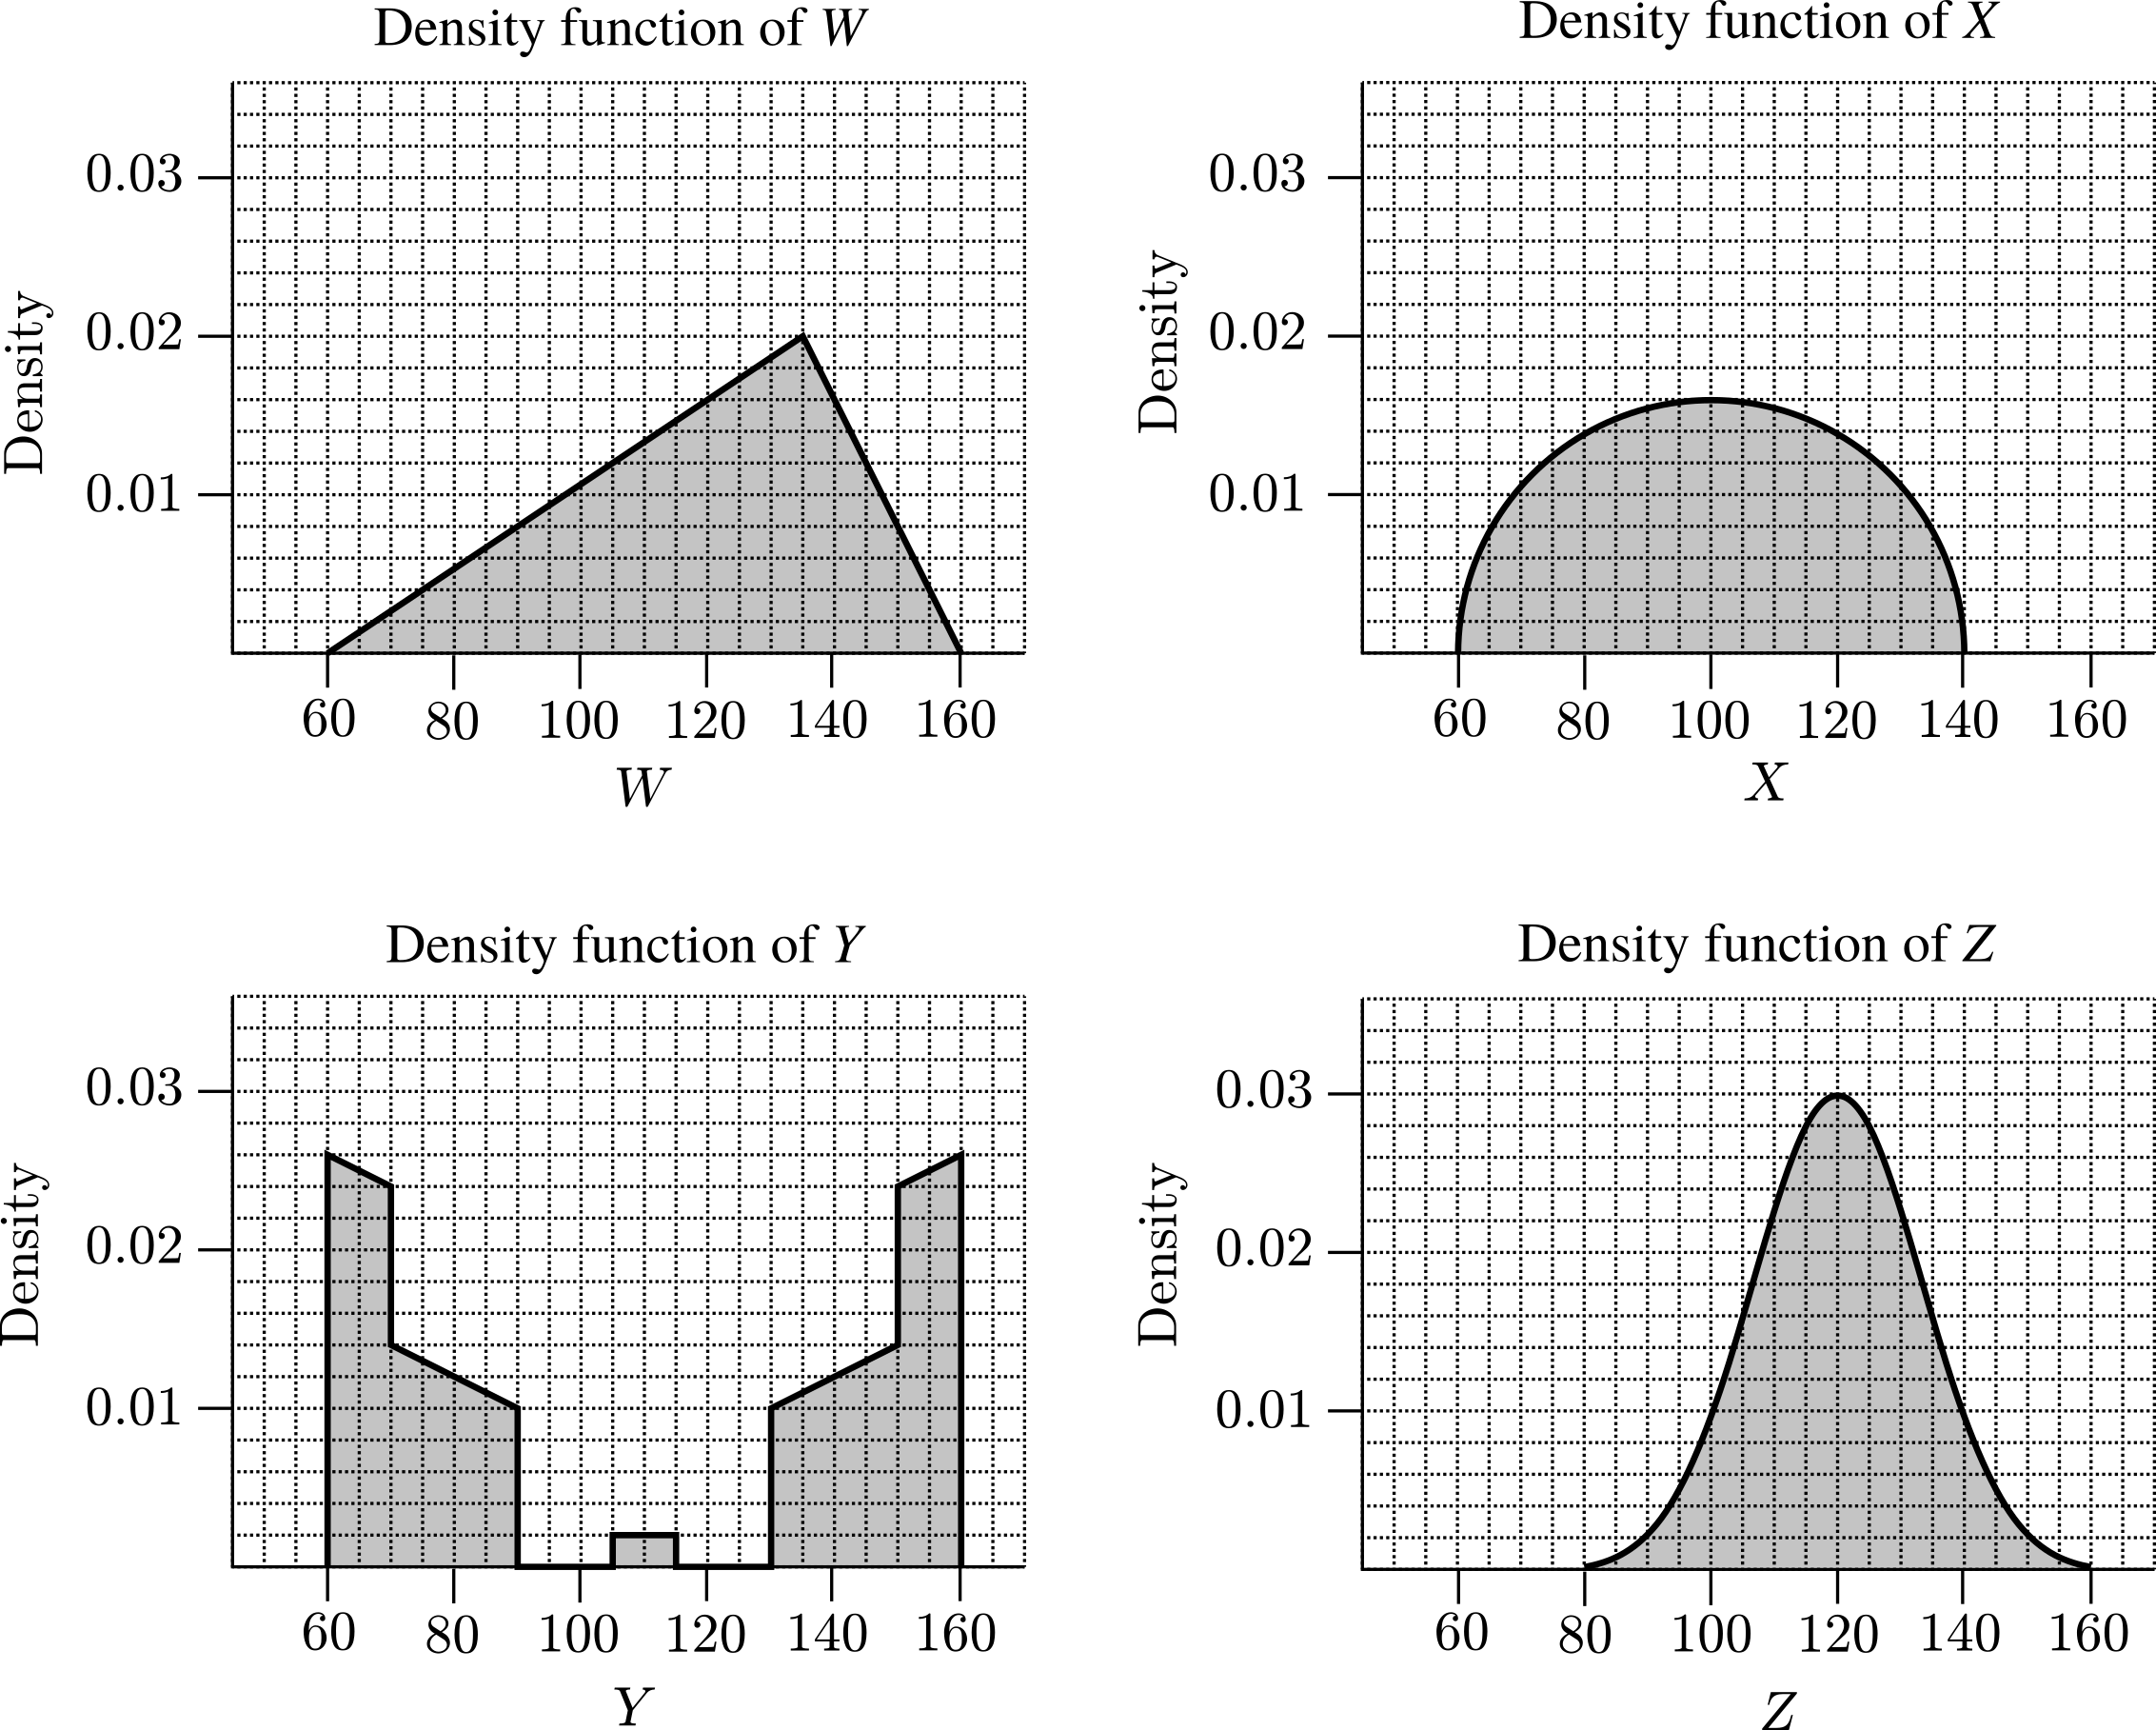
\includegraphics[scale=0.8]{figures/4_distros.png}
\end{center}
\begin{parts}
\part Which variable is most likely to fall below 100? \hfill
\makebox[0pt][r]{
\begin{oneparcheckboxes}
\choice $W$
\choice $X$
\choice $Y$
\choice $Z$
\end{oneparcheckboxes}}

\part Which distribution has the highest $Q_3$? \hfill
\makebox[0pt][r]{
\begin{oneparcheckboxes}
\choice $W$
\choice $X$
\choice $Y$
\choice $Z$
\end{oneparcheckboxes}}

\part Which variable is least likely to fall between 80 and 90? \hfill
\makebox[0pt][r]{
\begin{oneparcheckboxes}
\choice $W$
\choice $X$
\choice $Y$
\choice $Z$
\end{oneparcheckboxes}}

\part Which distribution has a mean not equal to its median? \hfill
\makebox[0pt][r]{
\begin{oneparcheckboxes}
\choice $W$
\choice $X$
\choice $Y$
\choice $Z$
\end{oneparcheckboxes}}

\part Which distribution has the smallest standard deviation? \hfill
\makebox[0pt][r]{
\begin{oneparcheckboxes}
\choice $W$
\choice $X$
\choice $Y$
\choice $Z$
\end{oneparcheckboxes}}

\part Which distribution has the largest standard deviation? \hfill
\makebox[0pt][r]{
\begin{oneparcheckboxes}
\choice $W$
\choice $X$
\choice $Y$
\choice $Z$
\end{oneparcheckboxes}}

\part Which variable is most likely to fall above 150? \hfill
\makebox[0pt][r]{
\begin{oneparcheckboxes}
\choice $W$
\choice $X$
\choice $Y$
\choice $Z$
\end{oneparcheckboxes}}

\part Which has a 8\% chance of falling between 95 and 100? \hfill
\makebox[0pt][r]{
\begin{oneparcheckboxes}
\choice $W$
\choice $X$
\choice $Y$
\choice $Z$
\end{oneparcheckboxes}}
\\

\part Using 50 draws from one of the above distributions, the following dot plot was made: \vspace{-0.7in}
\\
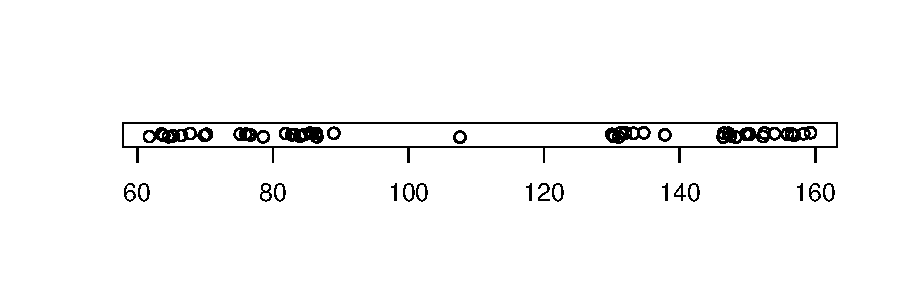
\includegraphics[scale=1]{figures/strip.pdf}
 \vspace{-0.5in}
 \\
 Which distribution was drawn from? \hfill
\makebox[0pt][r]{
\begin{oneparcheckboxes}
\choice $W$
\choice $X$
\choice $Y$
\choice $Z$
\end{oneparcheckboxes}}
 \\ 
 
\part $P(W=120) ~~=~~ ? $ \hfill
\makebox[0pt][r]{
\begin{oneparcheckboxes}
\choice $0$
\choice $0.016$
\choice $0.5$
\choice $1$
\end{oneparcheckboxes}}

\end{parts}

\newpage
\question[10] A study was done to investigate the relationship between $\rm{CO}_2$ and average temperature. The Mauna Lau observatory has continuously measured the concentration of $\rm{CO}_2$ over the last hundred years. Many other observatories have continuously measured temperature. Below we plot the two variables, where temperature is represented as degrees Celsius above expected (temperature anomaly).
\vspace{-0.7in}
\begin{center}
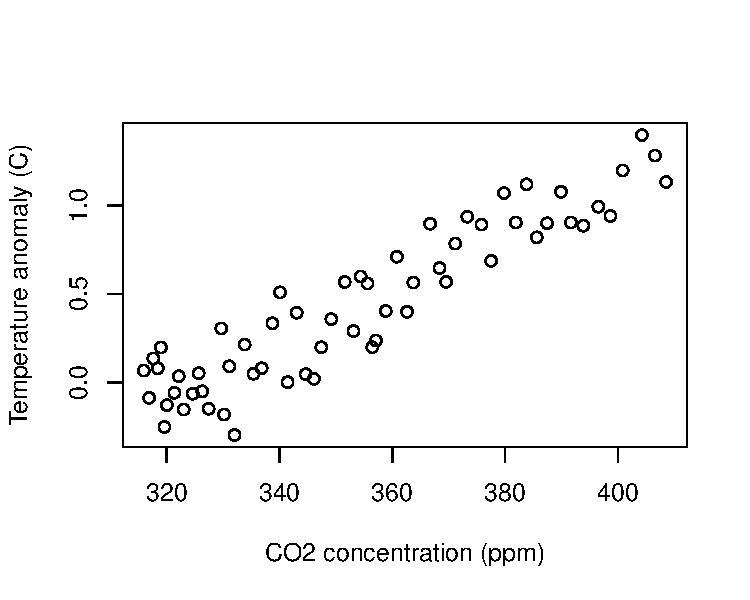
\includegraphics[scale=0.8]{figures/co2temp.pdf}
\end{center}
\begin{parts}
\part What kind of study was this (observational or experimental)?
\vfill
\part What is the implied explanatory variable?
\vfill
\part What is the implied response variable?
\vfill
\part What association is there between the two variables (positive, negative, or none)?
\vfill
\part Based on this study, should we conclude there is a causal relationship between the variables? 
\vfill
\part Suggest another possible hypothesis than ``more $\rm{CO}_2$ causes higher temperature anomalies''. For example, provide a possible confounding variable.
\vfill
\end{parts}

\newpage

\question[5] Complete the contingency table below by assuming $A$ and $B$ are {\bf independent} events.
\begin{center}\LARGE
\begin{tabular}{c|c c | c} 
     & ~~~$A$~~~ & ~~~$A^c$~~~ & total\\ \hline
$B$  & 0.1 &       & \\
$B^c$&     &       & \\ \hline
total &    &  0.6  & 1
\end{tabular}
\end{center}

\vfill

\question[5] A random sample of the bikes on Craiglist (near Boston in February) provided the following prices (in USD):
\begin{center}
\begin{tabular}{cccccccccc}
145 & 175 & 240 & 160 & 175 & 222 & 75 & 500 & 299 & 1300
\end{tabular}
\end{center}
Make a box plot summarizing these data.

\vfill

\newpage

\question [10] About 2.2\% of Boston commuters use bicycles. If a Boston commuter uses a bicycle, there is an 80\% chance their jacket is muddy. If a Boston commuter uses a nonbicycle, there is a 10\% chance their jacket is muddy. You see a Boston commuter with a muddy jacket and wonder if they commute via bicycle.
\begin{parts}
\part Draw a tree diagram.
\vfill
\vfill
\part Make a contingency table.
\vfill
\part Determine the probability the person commutes via bicycle given their jacket is muddy.
\vfill
\end{parts}

\newpage

\question[10] An urn contains marbles. Each marble has a color and a pattern. The frequencies are shown in the contingency table.
\begin{center}\large
\begin{tabularx}{0.8\textwidth}{|Y|Y Y Y|Y|}\hline
          & red & green & blue & total\\ \hline
dotted    & 18  & 24    & 15  & 57 \\
striped   & 32  & 16    & 23  & 71 \\
checkered & 27  & 19    & 30  & 76  \\ 
filled    & 15  & 22    & 16  & 53  \\ \hline
total     & 92  & 81    & 84  & 257 \\ \hline
\end{tabularx}
\end{center}
\begin{parts}
\part What is the probability that a random marble is red?
\vfill
\part What is the probability that a random marble is checkered?
\vfill
\part What is the probability that a random marble is blue and striped?
\vfill
\part What is the probability that a random marble is blue or striped?
\vfill
\part What is the probability that a random marble is striped given it is blue?
\vfill
\part What is the probability that a random marble is blue given it is striped?
\vfill
\end{parts}

\newpage

\question[10] The random variable $X$ follows the probability distribution below.
\vspace{10pt}

{\Large
\begin{tabular}{|c|c|}\hline 
$x_i$ & $P(X=x_i)$ \\ \hline
1 & 0.50\\
10 & 0.30\\
100 & 0.15\\
1000 & 0.05\\\hline
\end{tabular}
}

\vspace{10pt}
\begin{parts}
\part Evaluate $P(X = 100)$.
\vfill
\part Evaluate $P(10\le X \le 100)$.
\vfill
\part Evaluate the mean of the probability distribution. 
\vfill
\part Evaluate the standard deviation of the probability distribution. 
\vfill
\part Assume multiple draws are independent, where $X_i$ is the result of the $i$th draw. Evaluate the probability $P(X_1 = 10 \AND X_2 = 100)$. In other words, what is the chance of drawing a 10 and then a 100?
\vfill
\part Evaluate $P(X_1 \ne 1000 \AND X_2 \ne 1000 \AND  X_3 \ne 1000)$. In other words, what is the chance of drawing thrice and getting no 1000s?
\vfill
\part Evaluate $P(X_1 = 1000 \OR X_2 = 1000 \OR X_3 = 1000)$. In other words, what is the chance of drawing thrice and getting at least one 1000? 
\vfill
\end{parts}

\newpage

\question [10] A random sample was taken from a population. Each individual was measured, and those measurements are shown below.
\begin{center}
\begin{tabular}{cccccc}
62 & 48 & 55 & 24 & 51 & 60
\end{tabular}
\end{center}
\begin{parts}
\part Determine the sample mean.
\vfill
\part Determine the sample standard deviation.
\vfill
\end{parts}
\end{questions}
\end{document}